{% -*- mode: LaTeX; TeX-PDF-mode: t; TeX-master: "manual"; -*-
}

\chapter{\ei Clients}
\label{ch:clients}


The aim of the \ei clients is to facilitate the way users connect to
\ei servers, i.e., instead of directly using the protocol described in
Section~\ref{sec:server:access}, they can use a (graphical) user
interface that:
%
\begin{inparaenum}[\upshape(\itshape i\upshape)]
%
\item connects to the \ei servers and retrieves for the list of
  available tools;
%
\item allows the user to choose a tool to execute on some input files,
  and set the values of the corresponding parameters;
%
\item generates a corresponding request and sends it to a
  corresponding \ei server; and
%
\item shows the returned output to the user.
\end{inparaenum}
%
In addition, in some cases, clients are supposed to provide code
editing capabilities so user can edit their code as well in an
integrated developing environment.
%
In Section~\ref{sec:clients:web} we describe the web-client of the \ei
toolkit, and in Section~\ref{sec:clients:other} we discuss other
possible clients.
%


\section{Web-Interface Client}
\label{sec:clients:web}

\begin{figure}[h]
\hrule\smallskip
\begin{center}
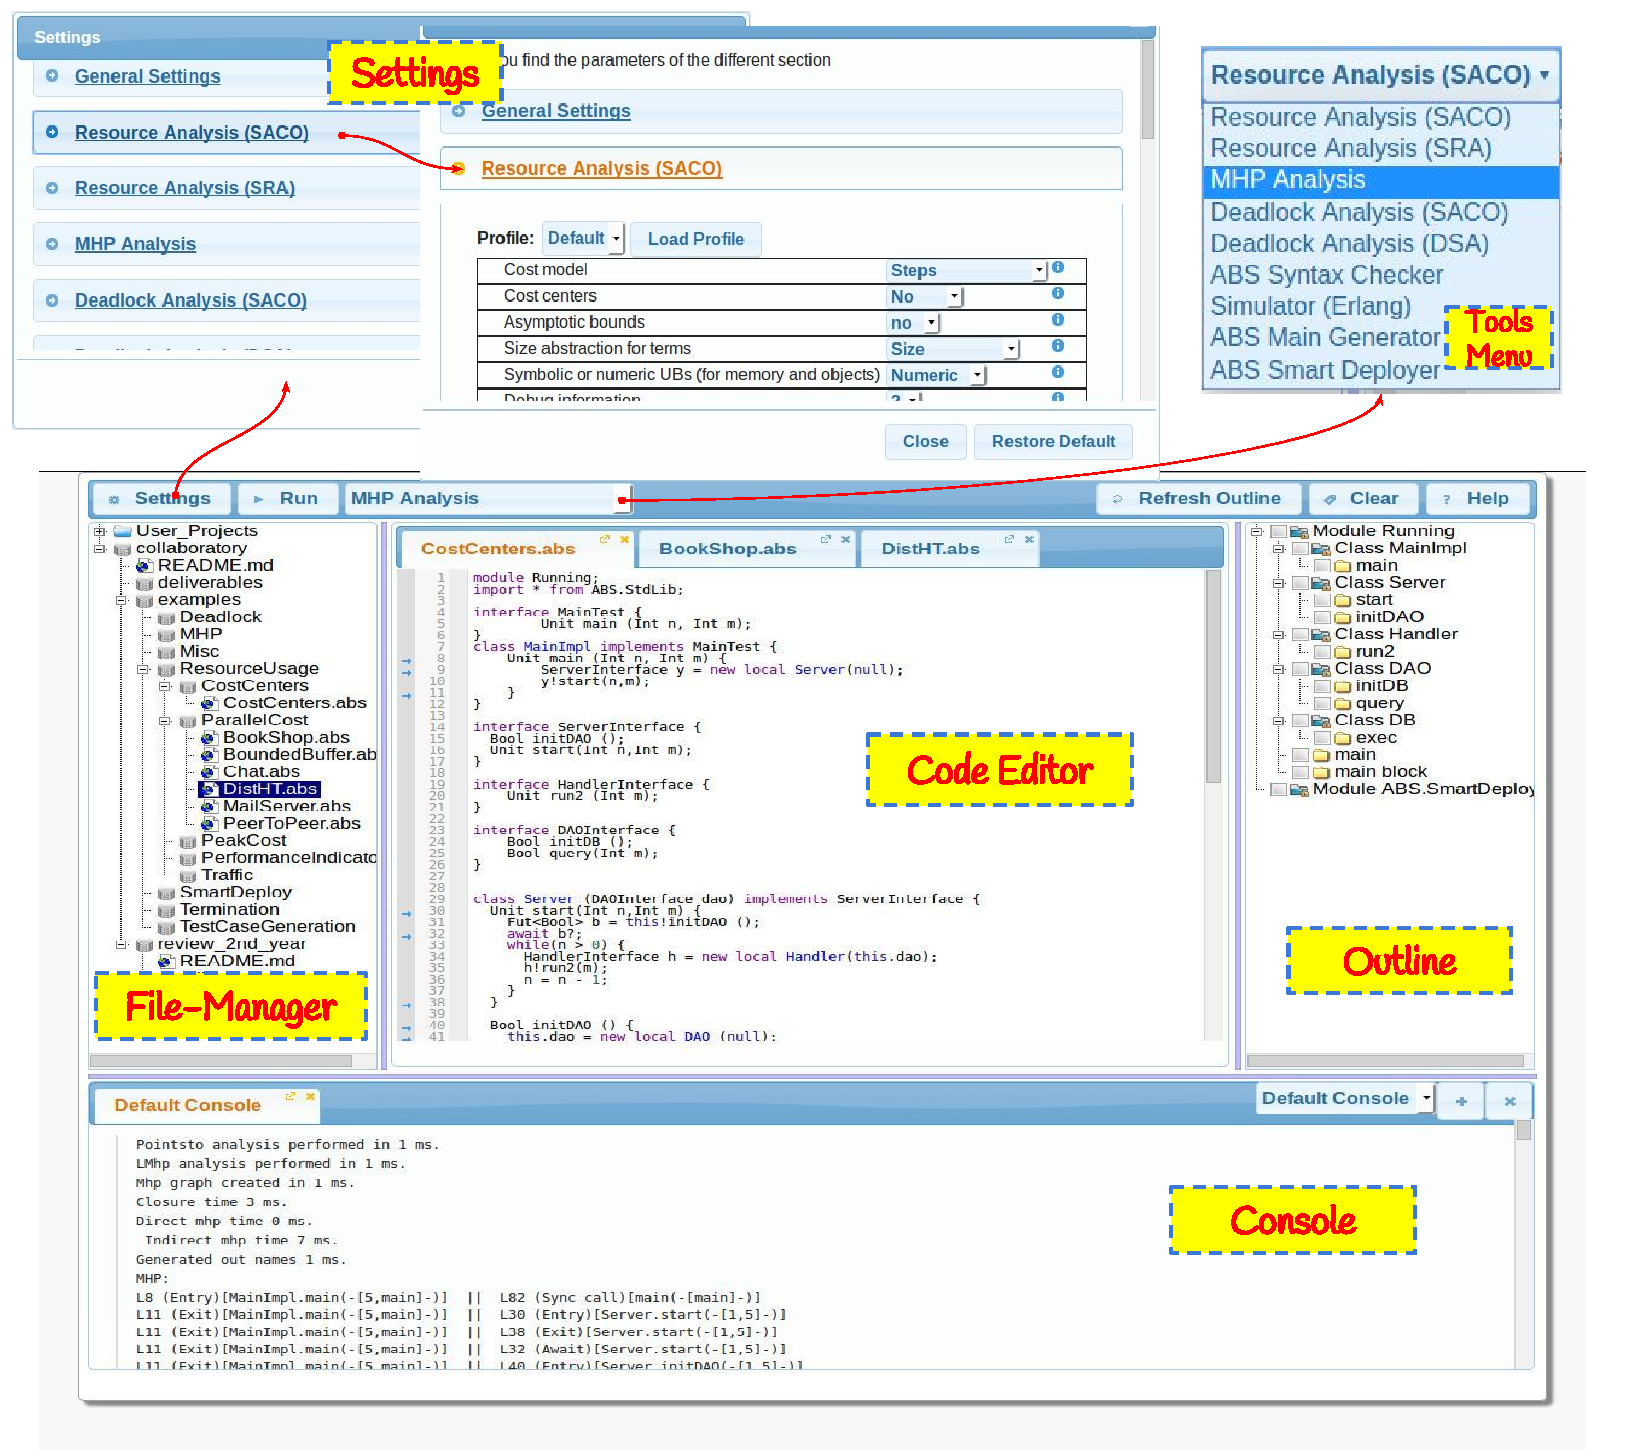
\includegraphics[width=1\textwidth]{fig/webclient2.pdf}
\end{center}
\caption{\ei Web Client}
\label{fig:clients:web}
\hrule
\end{figure}

The web-client of \ei is a JavaScript program that runs in a web
browser. It uses jQuery~\cite{jquery,steyer2013learning} as well as
some other libraries like jsTree~\cite{jstree} and
CodeMirror~\cite{codemirror}. It is part of the github repository
\url{http://github.com/abstools/easyinterface}, under the directory
\lst{clients/web}.
%
Once \ei is installed (see Appendix~\ref{ch:installation}), the
web-client can be accessed using
\url{http://localhost/ei/clients/web}. A representative screenshot of
the different parts of the web-client is depicted in
Figure~\ref{fig:clients:web}.
%
The web-client is designed like a development environment, and it
includes the following main components:
%
\begin{enumerate}
%
\item \lst{Code Editor}: an area were programs can be edited, which
  also provides the functionality of an editor in general such as
  \emph{search and replace} and \emph{syntax highlighting};
%
\item \lst{File Manager}: an area where users can manage their own
  files, and also access predefined sets of examples. In addition, it
  supports accessing GitHub repositories;
%
\item \lst{Outline}: an area where the different elements of the
  edited programs, such as class and method names, are shown. It is
  configurable depending on the programming languages used; 
%
\item \lst{Console}: an area where the output of a tool can be
  printed, which includes several tabs for better organization of the
  output; and
%
\item \lst{Settings}: an area where the parameters of each tool are
  viewed graphically, allowing users to set their values, or selecting
  a predefined profile, before running a tool.
%
\end{enumerate}
%
The interface has also a tool bar with a combo-box that includes the
list of available tools, a button to execute a tool, a button to
access the settings section, a button to create an outline, a button
to access the help section, and a button to clear the last output
generated.
%
The web-client includes an interpreter for the \ei output language
that is describe in Chapter~\ref{ch:eiol}.

The web-client can be easily configured to fit the user's needs, it
has a configuration file to control, among others, the following
aspects:
%
\begin{enumerate}[\upshape(\itshape i\upshape)]
\item the tools to include in the tools menu;
\item the examples to show in the file-manager; and
\item the tool be used for generating the outline for a set of
  programs -- note that this is programming language dependent).
\end{enumerate}
%
The web-client first looks for the configuration file
\lst{clients/web/webclient.cfg}, and if it does not exists it uses
\lst{$\mbox{clients/web/webclient.default.cfg}$} which is shipped by
default with \ei.
%
It is recommended not to directly modify
\lst{$\mbox{webclient.default.cfg}$}, but rather create a new copy
into \lst{webclient.cfg}.

Next we explain the different components of the configuration file. In
the rest of this chapter, when we refer the \emph{default server} we
mean the one that is available at the same address as the web-client,
i.e., if the web-client was accessed using the URL
%
\begin{center}
``\lst{http://somedomain/.../ei/client/web}'', 
\end{center}
%
then the URL of the default server is
%
\begin{center}
``\lst{http://somedomain/.../ei/server}''.
\end{center}
%
The configuration file is a text file that includes a single JSON
record with the following fields:

\bigskip
\begin{lstlisting}
{
  (*title:        ~~~~~~ \emph{A title to use for the window}*),
  (*apps:         ~~~~~~~ \emph{A list of tools to include in the tools menu}*),
  (*examples:     ~~~ \emph{A list of examples to include in the file manager}*),
  (*outline:      ~~~~ \emph{Indicates if the outline area should be hidden}*),
  (*outlineserver: \emph{The server of the tool for generating the outline}*),
  (*outlineapp:   ~ \emph{The name of the tool to generate outline}*)
  (*language:     ~~~ \emph{The programming language of the edited programs}*),
}
\end{lstlisting}%

\medskip
\noindent
All fields in the above record are optional, the web-client assigns
default values for those that are not available. Their meaning is as follows:
%
\begin{itemize}
\item \lst{$\mbox{title}$} is used to set the window title (see
  Figure~\ref{fig:clients:web}), where its default value is ``Easy
  Interface''.
%
\item \lst{$\mbox{apps}$} is used to change the set of tools to be
  listed in the tools menu, the syntax is explained in
  Section~\ref{sec:clients:web:toolsmenu}.
%
\item \lst{$\mbox{examples}$} is used to change the set of examples
  that are shown in the file-manager, the syntax is explained in
  Section~\ref{sec:clients:web:filemanager}.
%
\item \lst{$\mbox{outline}$} is use to control if the \lst{Outline}
  components (see Figure~\ref{fig:clients:web}) is visible or not, the
  possible values are ``\lst{on}'' and ``\lst{off}''.
%
\item \lst{$\mbox{outlineserver}$} and \lst{$\mbox{outlineapp}$} are
  used to indicate which tool to use for generating the content of the
  outline, the syntax is explained in
  Section~\ref{sec:clients:web:outline}.
%
\item \lst{$\mbox{language}$} is used to set the programming language
  in which programs are written (for syntax highlighting purposes),
  the syntax is explained in Section~\ref{sec:clients:web:codearea}.
\end{itemize}
%
In the next section we give some example values for these fields.


\subsection{Tools  Menu}
\label{sec:clients:web:toolsmenu}

The tool menu, the combo-box next to the \applybutton button in
Figure~\ref{fig:clients:web}, includes a list of tools that can be
executed by the user. This list can be modified by setting the value
of the field \lst{$\mbox{apps}$} in the configuration file. This value
is an array of JSON records of the form

\bigskip
\begin{lstlisting}
  { (*server: SRV, apps: APPSLIST*) }
\end{lstlisting}
 
\bigskip
\noindent  
where \lst{SVR} is a URL to an \ei server and \lst{APPSLIST} is an
array of tool identifiers (see \xmlstructref{server}{app}).
%
\lst{APPSLIST} can also be the special value \lst{_ei_all} which
refers to all tools of the corresponding server.
%
If this field is not provided, all tools from the default server will
be included in the tools menu.

\begin{example}
  The following is a possible value for field \lst{$\mbox{apps}$}:

\medskip
\begin{lstlisting}
(*apps: [~\{server: "http://domain1/ei/server, apps: ["costa", "mhp"]\},*)
(*~~~~~~~~~\{server: "http://domain2/ei/server, apps: "\_ei\_all"\} ]*)
\end{lstlisting}

\medskip
\noindent
It takes the tools identified by \lst{costa} and \lst{mhp} from the
\ei server \lst{http://domain1/ei/server}, and all tools available at
the \ei server \lst{http://domain2/ei/server}.

\end{example}

\subsection{File-Manger}
\label{sec:clients:web:filemanager}

In the file-manager area, of Figure~\ref{fig:clients:web}, we can see
a tree-view that represents programs on which tools can be applied,
etc. 
%
The one with the name \lst{User_Projects} corresponds to programs
that are created by the user; and the rest are predefined set of
examples. 
%
This set of examples can be modified by setting the value of the field
\lst{$\mbox{examples}$} in the configuration file. This value is an
array of JSON records of the form

\bigskip
\begin{lstlisting}
  { (*server: SRV, examples: EXLIST*) } 
\end{lstlisting}

\bigskip
\noindent
where \lst{SVR} is a URL to an \ei server and \lst{EXLIST} is an array
of example set identifiers (see \xmlstructref{server}{exset}).
%
\lst{EXLIST} can also be the special value \lst{_ei_all} which refers
to all example sets of the corresponding server.
%
If this field is not provided, all example sets from the default
server will be included.

\begin{example}
The following is a possible value for field \lst{$\mbox{examples}$}:

\medskip
\begin{lstlisting}
(*examples: [~\{server: "http://domain1/ei/server, examples: ["cost"]\},*)
(*~~~~~~~~~~~~\{server: "http://domain2/ei/server, examples: "\_ei\_all"\} ]*)
\end{lstlisting}

\medskip
\noindent
It takes the example set identified by \lst{cost} from the \ei server
\lst{http://domain1/ei/server}, and all example sets available at the
\ei server \lst{http://domain2/ei/server}.

\end{example}


Note that the file-manager has a context menu (use the mouse
right-click to open it) with options for: creating new files; running
tools; creating outline; cloning and committing to GitHub
repositories, etc.

\subsection{Outline}
\label{sec:clients:web:outline}

The outline area of Figure~\ref{fig:clients:web} includes a tree-view
that represents information on some programs entities, e.g., methods,
classes, etc. The actual values in this tree and its structure depend
very much on the intended use of \ei, and thus, it is completely
configurable -- apart from the possibility of hiding it by setting
\lst{outline} to ``\lst{off}''.
%
The idea is that the user will select some of the entries in this
tree, and then they will be passed to the tool that we run (see
Section~\ref{sec:quickguide:outline}
and~\xmlstructref{server}{cmdlineapp}).

The actual content of the outline is not generated by the web-client,
but rather by an external tool that is installed on some \ei server
that we refer to as the \emph{outline tool}. It is like any other tool
but typically non-visible.  The exact work-flow for generating an
outline is as follows:
%
\begin{enumerate}

\item The user clicks on the \refreshoutline button to generate an
  outline for the currently opened tab (in the code editor), or select
  the \refreshoutline option from the context menu of the file-manager
  to generate an outline for all programs in the corresponding
  sub-tree;

\item The web-client sends a request to execute the \emph{outline
    tool}, passing it all files of interest;

\item The \emph{outline tool} processes the input files and generates
  (on the standard output) some XML structure that represents the
  content of the outline, which is sent back to the client; and

\item The web-client converts this XML into a tree view as shown in
  Figure~\ref{fig:clients:web}.

\end{enumerate}
%
The fields \lst{outlineserver} and \lst{outlineapp} in the
configuration file can be used to indicate which tool to use for
generating the outline content. The default value of
\lst{outlineserver} is the default server, and the one of
\lst{outlineapp} is \lst{coutline} which a simple example tool
that comes with \ei to generate outlines for C programs.

As for the outline content, it must be \emph{a sequence of XML
  environments} that adhere to the following syntax, each element
(i.e., tree) in this sequence will be show at the root level in the
outline area:

%% 
\bigskip
\xmlstruct
{webclient}
{outline}
{%
%
  Defines a tree that represent (part of) an outline. The outer
  \lst{category} tag is the root of this tree, and the inner
  \xmlstructref{webclient}{outline}* are its children. The meaning of
  the different attributes is as follows:
%
\begin{itemize}
  \item \xmlstructattr{version} indicates the version of the outline
  structure, which is $1.0$ by default.
  \item \xmlstructattr{text} is the text to be show for that node.
  \item \xmlstructattr{value} is the value to passed to a tool if that node is selected.
  \item \xmlstructattr{selectable} indicates if this node can be
    selected. Its default value is \xmlstructvalue{true}. Such nodes
    are used to divide the tree in several logical categories.  Note
    that, in some clients, nodes might be still selectable even if the
    value is \xmlstructvalue{false}, however, in such case they will
    not be passed to the tool.
  \item \xmlstructattr{icon} is a URL to an alternative icon to be
    used for that node.
\end{itemize}
%
\bigskip
\noindent
\xmlstructdef{webclient}{nodetext}

A string.

\bigskip
\noindent
\xmlstructdef{webclient}{nodeval}

[a-z,A-Z,0-9,-,\_,:,.]+

\bigskip
\noindent
\xmlstructdef{webclient}{bool}

( \lst{true} | \lst{false} )

\bigskip
\noindent
\xmlstructdef{webclient}{url}

A valid \lst{http} or \lst{https} URL.
}

\begin{example}
%
The following is an example of a simple outline for an \abs program:

\medskip
\begin{lstlisting}
<category text="Module PingPong" selectable="false">
 <category text="Class PingImpl" selectable="false">
  <category text="initPing" value="PingImpl.initPing" selectable="true" />
  <category text="ping" value="PingImpl.ping" selectable="true" />
 </category>
 <category text="Class PongSessionImpl" selectable="false">
  <category text="initPongSession" value="PongSessionImpl.initPongSession" selectable="true" />
  <category text="pong" value="PongSessionImpl.pong" selectable="true" />
 </category>
 <category text="Class PongImpl" selectable="false">
  <category text="hello" value="PongImpl.hello" selectable="true" />
  <category text="sessionFinished" value="PongImpl.sessionFinished" selectable="true" />
 </category>
 <category text="main" value="main" selectable="true" />
</category>
\end{lstlisting}

\medskip
\noindent
It represent a module with three classes, each with several
methods. In addition, it includes a node representing the \lst{main}
block of the module. Note that only methods have the attribute
selectable set to \xmlstructvalue{true}. The result as viewed in the
web client is depicted in Figure~\ref{fig:clients:outline}.

\begin{figure}[t]
\hrule\smallskip
\begin{center}
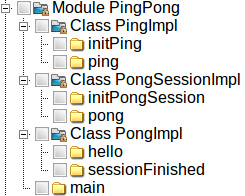
\includegraphics[width=.3\textwidth]{fig/outline.png}
\end{center}
\caption{Outline example}
\label{fig:clients:outline}
\hrule
\end{figure}

\end{example}

\subsection{Code Editor}
\label{sec:clients:web:codearea}

The \lst{Code Editor} in Figure~\ref{fig:clients:web} is the area
were programs can be edited. It provides basic functionality of an
editor in general such as \emph{search and replace} and \emph{syntax
  highlighting}.  It is implemented using the
CodeMirror~\cite{codemirror} library.
%
The syntax highlight is configurable via the field \lst{language} in
the configuration file.
%
Its value should be a valid CodeMirror syntax highlighting mode which
is a MIME%
\footnote{ \url{http://en.wikipedia.org/wiki/MIME}}
%
content-type attribute, for example: \emph{text/x-csrc} (C),
\emph{text/x-c++src} (C++), \emph{text/x-java} (Java),
\emph{text/x-csharp} (C\#), \emph{text/x-python} (Python), etc.  See
\url{http://codemirror.net/mode} for the list of available modes.
%
By default it is \emph{text/x-csrc}, i.e., C programs.
%
Note that CodeMirror provides an easy way to add new rules for syntax
highlighting as described in
\url{http://codemirror.net/doc/manual.html\#modeapi}. 
%
In such case, the new files should be incorporated in the local copy
of CodeMirror at \lst{clients/web/lib/codemirror/mode}.
%


\subsection{Console}
\label{sec:clients:web:console}

The console area is where the output of a tool can be printed, which
includes several tabs for better organization of the output. It is
implemented using jQuery~\cite{jquery}.

\subsection{Settings Section}
\label{sec:clients:web:settings}

The \lst{Settings} window in Figure~\ref{fig:clients:web} includes a
section for each available tool. In each section the parameters of the
corresponding tool (see \xmlstructref{server}{parameters}) are viewed
in a graphical way, e.g., using combo-boxes, radio buttons, etc.
%
One can select also a profile, which automatically sets the parameters
to some predefined values (see \xmlstructref{server}{profiles}). The
\emph{Default} profile sets all parameters to their default value.

\subsection{Help Section}
\label{sec:clients:web:help}

A click on the \helpbutton button in Figure~\ref{fig:clients:web} will
open a window that includes several help sections, one for each
tool. The content of each section is taken from the corresponding
tool's help provided in configuration file of the \ei server (see
\xmlstructref{server}{apphelp}).

\subsection{Other Features}
\label{sec:clients:web:other}

The web-client can be started directly with: some files (from the
file-manager) opened, a tool selected from the tools menu, and the
corresponding parameter set using some profile.
%
This is useful when writing, for example, tutorials for these tools,
where one can link directly to the web-client with a corresponding
example opened and a tool ready to be applied. 
%
This can be done using a URL of the following form:

\medskip
\begin{lstlisting}
$~~$ (*\mbox{http://domain/clients/web/?app=APPID\&profile=PROFILE\&file=PATH}*)
\end{lstlisting}

\medskip
\noindent
where: 
\begin{inparaenum}[\upshape(\itshape i\upshape)]
%
\item the value of \lst{$\mbox{app}$} is an identifier \lst{APPID} of
  the tool to be selected;
%
\item the value of each \lst{$\mbox{file}$} parameter (there can be
  several) is a \lst{PATH} to be opened in the editor --- it should be
  full path from the root of the file-manager, e.g.,
  ``\lst{/Examples_1/iterative/sum.c}''; and
%
\item the value of \lst{$\mbox{profile}$} is a profile identifier
  \lst{PROFILE} to be used for parameter values (see
  \xmlstructref{server}{profile}).
%
\end{inparaenum}
 
\section{Other Clients}
\label{sec:clients:other}

Although we have presented the web-client only, which is recognized as
the most important one in our objectives, other clients might be of
interest as well. For example, one can think of developing an Eclipse
plugin to communicate with a server within Eclipse, or a script
(e.g., Python) to communicate with a server within a terminal.
